\documentclass[11pt,a4paper]{article}

% ====== HO TRO TIENG VIET (pdfLaTeX hoac XeTeX/Tectonic) ======
\usepackage{iftex}
\ifPDFTeX
  \usepackage[utf8]{inputenc}
  \usepackage[T5]{fontenc}
\else
  \usepackage{fontspec}
  \setmainfont{Noto Serif}
  \setsansfont{Noto Sans}
  \setmonofont{Noto Sans Mono}
\fi
\usepackage[vietnamese]{babel}

\usepackage{amsmath,amssymb}
\usepackage{graphicx}
\usepackage{booktabs}
\usepackage{array}
\usepackage{float}
\usepackage{algorithm}
\usepackage{algpseudocode}   % thuoc goi algorithmicx
\algrenewcommand\textproc[1]{\textbf{#1}}
\usepackage{xcolor}
\usepackage{tikz}
\usetikzlibrary{calc,positioning,arrows.meta}
\definecolor{vizblue}{HTML}{2A78D6}
\definecolor{vizorange}{HTML}{EB6834}
\definecolor{vizaqua}{HTML}{1BAF7A}
\usepackage[hidelinks,unicode]{hyperref}
\usepackage{geometry}
\geometry{margin=2.5cm}

\floatname{algorithm}{Thuật toán}
\renewcommand{\listalgorithmname}{Danh sách thuật toán}

% ====== So lieu thuc nghiem (sinh tu dong tu results.json) ======
\newcommand{\NKeys}{100\,000}
\newcommand{\EnvPython}{3.14.4}
\newcommand{\EnvCPU}{Intel(R) Core(TM) i7-10700K CPU @ 3.80GHz}
\newcommand{\RuntimeSec}{20}
\newcommand{\FprThEight}{2.16\%}
\newcommand{\FprEmpEight}{2.16\%}
\newcommand{\FprThTen}{0.82\%}
\newcommand{\FprEmpTen}{0.82\%}
\newcommand{\KOptTen}{7}
\newcommand{\FillEmpTen}{0.503}
\newcommand{\FillThTen}{0.503}
\newcommand{\InsBFTen}{919}
\newcommand{\InsCBFTen}{438}
\newcommand{\QmissBFTen}{1\,377}
\newcommand{\QmissCBFTen}{1\,159}
\newcommand{\QhitBFTen}{748}
\newcommand{\QhitCBFTen}{552}
\newcommand{\DelCBFTen}{234}
\newcommand{\InsRatioTen}{2.10}
\newcommand{\QmissRatioTen}{1.19}
\newcommand{\MemBFTen}{125\,000}
\newcommand{\MemCBFFourTen}{500\,000}
\newcommand{\MemCBFEightTen}{1\,000\,000}
\newcommand{\BudgetBytes}{125\,000}
\newcommand{\EqFprBF}{0.82\%}
\newcommand{\EqFprCBFFour}{30.1\%}
\newcommand{\EqFprCBFEight}{54.9\%}
\newcommand{\EqCellsBF}{1\,000\,000}
\newcommand{\EqCellsCBFFour}{250\,000}
\newcommand{\EqCellsCBFEight}{125\,000}
\newcommand{\EqRatioFour}{37}
\newcommand{\EqRatioEight}{67}
\newcommand{\FnRatio}{8}
\newcommand{\FnK}{6}
\newcommand{\FnFpDeleted}{2\,164}
\newcommand{\FnPerformed}{2\,041}
\newcommand{\FnCount}{8\,063}
\newcommand{\FnRate}{8.06\%}


\begin{document}

\begin{titlepage}
    \centering
    \setlength\parindent{0cm}

    \vspace*{-1cm}
    \begin{tikzpicture}[overlay, remember picture]
        \draw[line width=3pt,color=black,fill=none]
            ($(current page.north west)+(2.5cm,-2cm)$) rectangle
            ($(current page.south east)-(1.5cm,-2.5cm)$);
        \draw[line width=1pt,color=black,fill=none]
            ($(current page.north west)+(2.65cm,-2.15cm)$) rectangle
            ($(current page.south east)-(1.65cm,-2.65cm)$);
    \end{tikzpicture}

    \fontsize{14pt}{16pt}\selectfont\textbf{HỌC VIỆN CÔNG NGHỆ BƯU CHÍNH VIỄN THÔNG}\par
    \vspace{0.3cm}
    \underline{\textbf{KHOA SAU ĐẠI HỌC}}\par

    \vspace{1cm}

    
\includegraphics[scale=0.25]{logo-PTIT.jpg}\par

    \vspace{1.4cm}
    \fontsize{20pt}{24pt}\selectfont\textbf{\MakeUppercase{Báo cáo chuyên đề}}\par

    \vspace{1cm}
    \fontsize{17pt}{20pt}\selectfont\textbf{So sánh Bloom Filter và Counting Bloom Filter\\
    trong bài toán lọc dữ liệu tốc độ cao}\par

    \vspace{1.1cm}
    \begin{center}
        \begin{minipage}{0.88\textwidth}
        \fontsize{12pt}{15pt}\selectfont
        \renewcommand{\arraystretch}{1.3}
        \begin{tabular}{@{}>{\bfseries}l >{\bfseries}l
                        @{\hspace{0.5em}--\hspace{0.5em}}l@{}}
        Giảng viên: & \multicolumn{2}{l@{}}{\textbf{TS. Đỗ Thanh Hà}} \\[0.8em]
        Học viên thực hiện: & NGUYỄN MẠNH CƯỜNG & B25CHHT082 \\
        & TRẦN DUY KHÁNH & B25CHHT100 \\
        & NGUYỄN ĐỨC HOÀNG & B25CHHT096 \\
        \end{tabular}
        \end{minipage}
    \end{center}

    \vfill
    \fontsize{12pt}{14pt}\selectfont\textbf{HÀ NỘI -- 2026}\par
    \vspace{0.5cm}
\end{titlepage}

\tableofcontents
\listoffigures
\listoftables
\newpage

\section*{Danh mục ký hiệu và chữ viết tắt}
\addcontentsline{toc}{section}{Danh mục ký hiệu và chữ viết tắt}
\begin{center}
\renewcommand{\arraystretch}{1.2}
\begin{tabular}{@{}l>{\raggedright\arraybackslash}p{0.68\textwidth}@{}}
\toprule
Ký hiệu / viết tắt & Ý nghĩa \\
\midrule
$m$ & số ô của bộ lọc (bit với BF; counter với CBF) \\
$n$ & số phần tử đã chèn vào bộ lọc \\
$n'$ & số khóa vắng mặt dùng để đo FPR \\
$k$ & số hàm băm; $k^{*}=(m/n)\ln 2$ là giá trị tối ưu \\
$p$ & xác suất dương tính giả \\
$b$ & độ rộng một counter của CBF, tính bằng bit (mặc định $b=4$) \\
$C[i]$ & giá trị counter thứ $i$ của CBF \\
$\lambda$ & kỳ vọng số lượt băm vào một ô, $\lambda=kn/m$ \\
BF & Bloom Filter \\
CBF & Counting Bloom Filter (4-bit/8-bit chỉ độ rộng counter) \\
FPR & false positive rate (tỉ lệ dương tính giả) \\
KTC & khoảng tin cậy (trong báo cáo: khoảng Wilson, mức 95\%) \\
IQR & interquartile range (khoảng tứ phân vị của các lượt đo) \\
DPI / IDS & deep packet inspection / intrusion detection system \\
LSM-tree, SSTable & cây log-structured merge; tệp bảng sắp xếp bất biến \\
payload & phần dữ liệu chính của mảng lưu trữ, không tính overhead \\
contract của delete & tiền điều kiện: chỉ xóa khóa chắc chắn đã chèn \\
\bottomrule
\end{tabular}
\end{center}
\newpage

\begin{abstract}
Báo cáo so sánh Bloom Filter (BF, Bloom 1970) và Counting Bloom Filter (CBF,
Fan \emph{et al.} 2000) cho bài toán lọc dữ liệu tốc độ cao (lọc gói tin,
deep packet inspection, lọc truy vấn cơ sở dữ liệu, lọc cache, khử trùng lặp).
Chúng tôi trình bày cơ sở lý thuyết, công thức xác suất dương tính giả (false
positive), phân tích tràn counter, mã giả cho các thao tác insert/query/delete,
và một bộ thực nghiệm Python tự cài đặt cả hai cấu trúc. Kết quả trên
$n=\NKeys{}$ khóa xác nhận: (i) tỉ lệ dương tính giả (FPR) thực nghiệm bám sát
công thức $p=(1-e^{-kn/m})^k$ và khi dùng cùng bộ hàm băm, cùng $m$, $k$ thì BF
và CBF cho kết quả truy vấn \emph{trùng nhau từng khóa}; (ii) phần dữ liệu
chính (payload) của CBF 4-bit tốn đúng $4\times$ BF, do đó với cùng ngân
sách byte, FPR của CBF (\EqFprCBFFour{}) cao hơn BF (\EqFprBF{}) khoảng
\EqRatioFour{} lần, tức hơn một bậc độ lớn; (iii) CBF hỗ trợ
xóa an toàn khi bên gọi (caller) chỉ xóa khóa chắc chắn đã chèn: xóa đúng
\FnValidDeleted{} khóa không làm mất khóa thật nào còn lại, trong khi stress
test trên một bộ lọc riêng chứa đủ $n$ khóa, cố ý xóa các false positive,
tạo ra \FnCount{} false negative (\FnRate{} của $n$); (iv)~ở cùng mức
${\approx}10$ bit/khóa, trong các cấu trúc hỗ trợ xóa, Cuckoo Filter đạt
FPR \CkFpr{}, thấp hơn CBF 4-bit hơn một bậc độ lớn. Kết luận: dùng BF
cho tập gần như tĩnh; dùng CBF khi cần xóa động
và hệ thống bảo đảm được contract của delete; khi cần xóa với FPR mục tiêu
$<3\%$, Cuckoo Filter là lựa chọn đáng cân nhắc hơn.
\end{abstract}

\section{Giới thiệu}
Lọc dữ liệu tốc độ cao quy về bài toán \emph{kiểm tra thành viên tập hợp xấp
xỉ} (approximate set-membership): cho tập $S$ và khóa $x$ (gói tin, chữ ký mã
độc, khóa cơ sở dữ liệu, fingerprint khối dữ liệu), cần trả lời nhanh ``$x$
\emph{chắc chắn không} thuộc $S$'' hoặc ``$x$ \emph{có thể} thuộc $S$'' với
ngân sách bộ nhớ đủ nhỏ để nằm gọn trong SRAM/cache. Việc chấp nhận một tỉ lệ
nhỏ dương tính giả cho phép giảm mạnh không gian lưu trữ so với bảng băm chính
xác. Đây là đánh đổi không gian/thời gian kinh điển của
Bloom~\cite{bloom1970}.

Các miền ứng dụng tiêu biểu gồm: (i) \emph{lọc gói tin và DPI/IDS}: đối sánh
chữ ký Snort bằng Bloom filter song song trên FPGA~\cite{dpi2003}; (ii)
\emph{lọc truy vấn cơ sở dữ liệu} kiểu LSM-tree: RocksDB có thể gắn một BF cho
mỗi SSTable để bỏ qua các tệp ``chắc chắn không chứa khóa'', tránh I/O
đĩa~\cite{rocksdbBloom}; (iii) \emph{web cache hợp tác}: Cache Digest của Squid và giao thức
Summary Cache~\cite{fan2000}; (iv) \emph{khử trùng lặp} (deduplication) trên
fingerprint khối dữ liệu.

Đóng góp của báo cáo: hệ thống hóa lý thuyết BF/CBF; cài đặt độc lập cả hai
cấu trúc (kể cả CBF 4-bit đóng gói nibble đúng nghĩa); và bộ thực nghiệm định
lượng bốn khía cạnh: độ chính xác, thông lượng, bộ nhớ, và rủi ro false
negative khi xóa.

\section{Cơ sở lý thuyết}
\subsection{Bloom Filter (Bloom, 1970)}
BF gồm mảng $B$ có $m$ bit khởi tạo $0$ và $k$ hàm băm độc lập, phân bố đều
$h_1,\dots,h_k:\mathcal{U}\to\{0,\dots,m-1\}$. \emph{Insert}$(x)$ đặt
$B[h_i(x)]=1$ với mọi $i$; \emph{Query}$(x)$ trả ``có thể có'' nếu mọi bit
tương ứng bằng $1$, ngược lại trả ``chắc chắn không''. Bit đã bật không bao
giờ tự tắt nên BF \textbf{không có false negative}, nhưng \textbf{có false
positive} do va chạm băm. BF \textbf{không hỗ trợ xóa}: tắt các bit của $x$
có thể tắt nhầm bit đang được phần tử khác dùng chung.

\subsection{Counting Bloom Filter (Fan \emph{et al.}, 2000)}
CBF thay mỗi bit bằng một \emph{counter} $b$ bit (thường $b=4$), ký hiệu
$C[i]$. \emph{Insert} tăng, \emph{Delete} giảm $k$ counter tương ứng;
\emph{Query} trả ``có thể có'' khi mọi counter dương. Contract của Delete yêu
cầu bên gọi (caller) chỉ xóa khóa chắc chắn đã chèn: câu trả lời ``có thể có'' của Query
không chứng minh membership và không thể dùng làm điều kiện đủ để xóa. Khi
contract này được tuân thủ và counter không mất thông tin do tràn, CBF không
sinh false negative. Hai nguồn phá vỡ bảo đảm là \emph{tràn counter} khi hơn
$2^b-1$ phần tử băm vào cùng một ô, và \emph{xóa sai} một phần tử chưa từng
chèn~\cite{fan2000,broder2004}.

\subsection{Công thức xác suất}
\label{sec:formulas}
Sau khi chèn $n$ phần tử với $k$ hàm băm, xác suất một bit cụ thể còn $0$:
\begin{equation}
p_0=\left(1-\tfrac{1}{m}\right)^{kn}\approx e^{-kn/m}.
\end{equation}
Xác suất dương tính giả (cả $k$ bit của một khóa lạ đều bằng 1):
\begin{equation}
\label{eq:fpr}
p \;\approx\; \left(1-e^{-kn/m}\right)^{k}.
\end{equation}
Cực tiểu hóa $p$ theo $k$ (tương đương yêu cầu tỉ lệ bit $0$ bằng $1/2$,
tức entropy cực đại) cho số hàm băm tối ưu và bộ nhớ tối ưu theo FPR mục tiêu $p$:
\begin{equation}
\label{eq:kopt}
k^{*}=\frac{m}{n}\ln 2\approx 0.693\,\frac{m}{n},\qquad
m=-\frac{n\ln p}{(\ln 2)^{2}}\;\Longleftrightarrow\;
\frac{m}{n}\approx 1.44\log_2\frac{1}{p}.
\end{equation}
Tại $k^{*}$: $p=2^{-(m/n)\ln 2}\approx 0.6185^{\,m/n}$. Quy tắc thực dụng:
$m/n=8$ cho FPR $\approx 2\%$; $m/n=10$ cho FPR $<1\%$.

\paragraph{Dẫn xuất công thức~(\ref{eq:fpr}).}
Mỗi lần băm chọn một trong $m$ ô với xác suất đều nhau, nên một ô cụ thể
\emph{không} bị chọn với xác suất $1-1/m$. Chèn $n$ phần tử với $k$ hàm băm
tạo ra $kn$ lần băm độc lập, do đó một bit cụ thể vẫn bằng $0$ với xác suất
$(1-1/m)^{kn}$; dùng giới hạn kinh điển $(1-1/m)^{m}\to e^{-1}$ khi $m$ lớn
ta được xấp xỉ $e^{-kn/m}$ trong~(1). Một khóa lạ bị báo nhầm ``có'' khi cả
$k$ vị trí của nó đều mang bit 1; xấp xỉ coi $k$ bit này độc lập cho
ra~(\ref{eq:fpr}). Cần lưu ý hai điểm: (i)~các bit không hoàn toàn độc lập,
nên~(\ref{eq:fpr}) chỉ là xấp xỉ và trên thực tế là \emph{cận dưới} của FPR
thật; độ chệch thấy rõ nhất khi bộ lọc dày đặc ($m/n$ nhỏ), điều mà thực
nghiệm ở Mục~\ref{sec:e1result} quan sát được trực tiếp; (ii)~phân tích giả
định hàm băm lý tưởng, phân bố đều.

\paragraph{Dẫn xuất số hàm băm tối ưu.}
Lấy logarit của~(\ref{eq:fpr}): $\ln p = k\ln\!\left(1-e^{-kn/m}\right)$.
Đặt $t=e^{-kn/m}$ (tỉ lệ bit 0 kỳ vọng), khi đó $k=-(m/n)\ln t$ và
$\ln p = -(m/n)\ln t\,\ln(1-t)$. Biểu thức $\ln t\,\ln(1-t)$ đối xứng qua
$t=1/2$ và đạt cực đại tại đó, nên $p$ đạt cực tiểu khi $t=1/2$: nghĩa là
bộ lọc tối ưu có \emph{một nửa số bit bằng 0}, tức trạng thái entropy cực
đại, khi mỗi bit mang lượng thông tin lớn nhất. Thay $t=1/2$ vào $k=-(m/n)\ln t$
được $k^{*}=(m/n)\ln 2$, và $p=2^{-k^{*}}$ cho vế còn lại
của~(\ref{eq:kopt}). Bảng~\ref{tab:theory} liệt kê vài giá trị tiêu biểu;
sáu dòng đầu chính là các cấu hình được kiểm chứng thực nghiệm ở
Mục~\ref{sec:e1result}.

\begin{table}[H]\centering
\caption{Giá trị lý thuyết: số hàm băm tối ưu và FPR theo tỉ lệ $m/n$}
\label{tab:theory}
\begin{tabular}{@{}rrr@{}}
\toprule
$m/n$ & $k^{*}=\mathrm{round}((m/n)\ln 2)$ & FPR tại $k^{*}$\\
\midrule
4  & 3  & 14.689\% \\
6  & 4  & 5.606\% \\
8  & 6  & 2.158\% \\
10 & 7  & 0.819\% \\
12 & 8  & 0.314\% \\
16 & 11 & 0.046\% \\
20 & 14 & 0.007\% \\
\bottomrule
\end{tabular}
\end{table}

\paragraph{Từ hai hàm băm đến $k$ vị trí.}
Tính $k$ hàm băm độc lập cho mỗi khóa là tốn kém. Sơ đồ double hashing của
Kirsch--Mitzenmacher~\cite{kirsch2008} chỉ cần hai hàm băm $h_1,h_2$ rồi
sinh $k$ vị trí bằng $g_i(x)=(h_1(x)+i\,h_2(x)) \bmod m$; phân tích chứng
minh FPR tiệm cận không đổi so với $k$ hàm độc lập. Một chi tiết cài đặt
quan trọng: nếu $\gcd(h_2,m)>1$ (trường hợp xấu nhất là $h_2\equiv 0$), dãy
$g_i$ suy biến và chỉ phủ một phần mảng; buộc $h_2$ nhận giá trị lẻ loại trừ
rủi ro này với mọi $m$ chẵn (kể cả lũy thừa của 2), tương ứng với phép
\texttt{h2 |= 1} trong bản cài đặt của chúng tôi
(notebook \texttt{thuc\_nghiem.ipynb}).

\paragraph{Tràn counter và vì sao 4 bit là đủ.}
Số phần tử băm vào một counter tuân theo phân bố nhị thức
$\mathrm{B}(nk,1/m)\approx\mathrm{Poisson}(\lambda)$ với $\lambda=kn/m=\ln 2$
ở cấu hình tối ưu. Do đó
\begin{equation}
\Pr[C[i]=16]\approx \frac{e^{-\ln 2}(\ln 2)^{16}}{16!}\approx
6.78\times10^{-17},
\end{equation}
và Fan \emph{et al.} chặn trên toàn cục: với $k\le(\ln 2)m/n$,
$\Pr[\max_i C[i]\ge 16]\le m\cdot 1.37\times10^{-15}$~\cite{fan2000}. Vì
xác suất này vô cùng nhỏ (``minuscule''), counter 4 bit (đếm $0..15$) đủ cho
hầu hết ứng dụng. CBF tốn $4\times$ payload so với BF cùng số ô~\cite{broder2004}.
Nếu insert bão hòa ở 15 rồi delete vẫn giảm như counter thường, số lần tăng
vượt ngưỡng đã bị mất và false negative có thể xuất hiện sau nhiều lần xóa.
Chính sách ``sticky saturation'' (không bao giờ giảm ô đã bão hòa) tránh lỗi
này nhưng đổi lại tạo false positive dai dẳng; do đó hệ thống thực tế cần
theo dõi overflow hoặc rebuild từ nguồn dữ liệu chuẩn (source of truth).

\paragraph{Hai hệ quả cho việc so sánh.}
(1)~Với \emph{cùng} $m$, $k$ và cùng bộ hàm băm, một ô của CBF dương khi và
chỉ khi bit tương ứng của BF bằng 1 (khi chỉ chèn, chưa xóa), nên hai cấu
trúc trả lời truy vấn \emph{giống hệt nhau từng khóa}; CBF không ``chính
xác hơn'' BF. (2)~Với \emph{cùng ngân sách byte}, BF có số ô gấp $b$ lần CBF
$b$-bit, nên FPR của BF luôn thấp hơn hẳn (Mục~\ref{sec:equalbudget}).

\section{Mã giả}
\begin{algorithm}[H]
\caption{Bloom Filter: Insert và Query}
\begin{algorithmic}[1]
\Procedure{BF-Insert}{$x$}
  \For{$i \gets 1$ \textbf{to} $k$} \State $B[h_i(x)] \gets 1$ \EndFor
\EndProcedure
\Procedure{BF-Query}{$x$}
  \For{$i \gets 1$ \textbf{to} $k$}
     \If{$B[h_i(x)] = 0$} \State \Return \texttt{False} \Comment{chắc chắn không}
     \EndIf
  \EndFor
  \State \Return \texttt{True} \Comment{có thể có}
\EndProcedure
\end{algorithmic}
\end{algorithm}

\begin{algorithm}[H]
\caption{Counting Bloom Filter: Insert, Query, Delete (insert bão hòa)}
\begin{algorithmic}[1]
\Procedure{CBF-Insert}{$x$}
  \For{$i \gets 1$ \textbf{to} $k$}
     \If{$C[h_i(x)] < 2^{b}-1$} \State $C[h_i(x)] \gets C[h_i(x)]+1$
     \EndIf \Comment{bão hòa ở $2^b-1$}
  \EndFor
\EndProcedure
\Procedure{CBF-Query}{$x$}
  \For{$i \gets 1$ \textbf{to} $k$}
     \If{$C[h_i(x)] = 0$} \State \Return \texttt{False} \EndIf
  \EndFor
  \State \Return \texttt{True}
\EndProcedure
\Procedure{CBF-Delete}{$x$}
  \State \textbf{Tiền điều kiện:} caller biết $x$ đã được chèn
  \For{$i \gets 1$ \textbf{to} $k$}
     \If{$C[h_i(x)] > 0$} \State $C[h_i(x)] \gets C[h_i(x)]-1$
     \EndIf
  \EndFor
\EndProcedure
\end{algorithmic}
\end{algorithm}

\section{So sánh định tính}
\begin{table}[H]\centering
\caption{So sánh Bloom Filter và Counting Bloom Filter}
\label{tab:qualitative}
\small
\begin{tabular}{@{}
  >{\raggedright\arraybackslash}p{0.24\textwidth}
  >{\raggedright\arraybackslash}p{0.28\textwidth}
  >{\raggedright\arraybackslash}p{0.40\textwidth}@{}}
\toprule
Tiêu chí & Bloom Filter & Counting Bloom Filter \\
\midrule
Đơn vị ô          & 1 bit                  & counter $b$ bit ($b{=}4$) \\
Bộ nhớ payload    & $m$ bit                & $b\cdot m$ bit ($\sim4\times$) \\
Xóa (delete)      & Không                  & Có, với khóa biết chắc đã chèn \\
False positive    & Có, $p\approx(1-e^{-kn/m})^k$ & Có (cùng công thức) \\
False negative    & Không bao giờ          & Không nếu dùng đúng; có thể khi tràn/xóa sai \\
Insert/Query      & $O(k)$                 & $O(k)$ \\
FPR cùng ngân sách byte & Thấp hơn ($b\times$ số ô) & Cao hơn \\
Song song hóa cập nhật & Ghi 1 bit an toàn & Đọc--sửa--ghi cần đồng bộ \\
Hợp phần cứng     & Rất tốt (SRAM on-chip) & Tốn SRAM hơn (thường ở phần mềm) \\
Ứng dụng điển hình & SSTable filter, Cache Digest, & Router xóa flow, cache động, \\
                   & chữ ký DPI tĩnh, dedup & Summary Cache cục bộ \\
\bottomrule
\end{tabular}
\end{table}

\section{Ứng dụng trong lọc dữ liệu tốc độ cao}
\label{sec:applications}
Trước khi vào thực nghiệm, mục này đối chiếu đặc tính BF/CBF với bốn miền
ứng dụng tiêu biểu; mỗi miền minh họa một cách phân vai khác nhau giữa cấu
trúc gọn nhẹ không hỗ trợ xóa (BF) và cấu trúc hỗ trợ xóa với chi phí bộ
nhớ cao hơn (CBF).

\subsection{Deep packet inspection và IDS}
Dharmapurikar \emph{et al.}~\cite{dpi2003} đặt các Bloom filter \emph{song
song} trong SRAM on-chip của FPGA, mỗi bộ lọc phụ trách một độ dài chữ ký;
tại mỗi vị trí byte của luồng dữ liệu, mọi độ dài được kiểm tra đồng thời.
Chỉ khi một filter báo ``có thể có'', gói tin mới được chuyển sang khối so
khớp chính xác; nhờ đó BF đóng vai trò \emph{lọc thô}, loại bỏ phần lớn lưu lượng
vô hại ở tốc độ đường truyền. Nguyên mẫu trên Xilinx Virtex~2000E hỗ trợ
khoảng 10\,000 chữ ký với thông lượng ${\sim}600$~Mbps; các thiết kế phần
cứng kế tiếp cùng hướng nhắm tới hàng chục Gbps. Tập chữ ký IDS ít thay đổi
nên BF thuần phù hợp; khi cần cập nhật, mô hình lai thường dùng là CBF trong
phần mềm điều khiển (nơi giữ nguồn dữ liệu chuẩn, nên delete tuân thủ
contract như E4 đòi hỏi) và BF phần cứng được đồng bộ lại từ đó.

\subsection{Lọc truy vấn trong cơ sở dữ liệu LSM-tree}
Trong RocksDB, mỗi tệp SSTable (bất biến sau khi ghi) mang một Bloom filter
riêng; truy vấn điểm kiểm tra filter trước, câu trả lời ``chắc chắn không''
cho phép bỏ qua tệp mà không tốn I/O đĩa~\cite{rocksdbBloom}, qua đó giảm trực
tiếp read amplification. Đáng chú ý, tính bất biến của SSTable khiến nhu cầu
xóa khỏi filter \emph{không tồn tại}: compaction tạo tệp mới kèm filter mới,
đúng chiến lược ``rebuild thay vì delete'' mà Mục~\ref{sec:recommend}
khuyến nghị. Cấu hình phổ biến khoảng 10~bit/khóa cho FPR quanh 1\%, khớp
Bảng~\ref{tab:theory}; bản full filter hiện đại còn gói toàn bộ probe vào
một cache line (Mục~\ref{sec:variants}).

\subsection{Web cache hợp tác}
Giao thức Summary Cache~\cite{fan2000}, nơi CBF ra đời, cho mỗi proxy
giữ \emph{tóm tắt} thư mục cache của các proxy láng giềng dưới dạng BF, và
chỉ chuyển tiếp yêu cầu khi tóm tắt báo ``có thể có''. Vì nội dung cache
thay đổi liên tục, mỗi proxy duy trì một CBF \emph{cục bộ} cho thư mục của
chính mình (đủ thông tin để xóa an toàn) và định kỳ phát snapshot dạng BF
0/1 cho láng giềng: CBF đứng ở nơi có nguồn dữ liệu chuẩn, BF đứng ở nơi chỉ
cần tra cứu. Fan \emph{et al.} báo cáo giảm số thông điệp liên proxy
25--60 lần và băng thông hơn 50\% so với giao thức ICP truyền thống, với
load factor $m/n$ từ 8 đến 16~\cite{fan2000}. Cache Digest của Squid dùng
cùng nguyên lý.

\subsection{Khử trùng lặp dữ liệu}
Hệ thống sao lưu/khử trùng lặp băm mỗi khối dữ liệu thành fingerprint và
giữ chỉ mục đầy đủ trên đĩa; một BF trong RAM trả lời ``chắc chắn chưa
gặp'' giúp ghi khối mới không cần tra chỉ mục~\cite{broder2004}. False
positive ở đây chỉ gây một lần tra cứu thừa, không ảnh hưởng đúng đắn. Khi
có thu hồi khối (garbage collection), tập fingerprint co lại; khi đó hoặc dùng
CBF, hoặc đơn giản rebuild filter theo chu kỳ thu hồi.

\section{Phương pháp thực nghiệm}
\label{sec:method}
\paragraph{Môi trường.} Python \EnvPython{}, CPU \EnvCPU{}; các gói
\texttt{mmh3} \EnvMmhThree{}, \texttt{bitarray} \EnvBitarray{},
\texttt{matplotlib} \EnvMatplotlib{}, \texttt{numpy} \EnvNumpy{} và
\texttt{pandas} \EnvPandas{}. Toàn bộ mã thực nghiệm nằm trong notebook
\texttt{thuc\_nghiem.ipynb}; chạy hết \RuntimeSec{} giây.

\paragraph{Cài đặt.} Ba cấu trúc được cài đặt từ đầu
(notebook \texttt{thuc\_nghiem.ipynb}): \textbf{BF} dùng mảng bit
(\texttt{bitarray}); \textbf{CBF 4-bit} đóng gói 2 counter/byte (nibble
packing), đúng chi phí $4\times$ như phân tích lý thuyết; \textbf{CBF
8-bit} dùng counter đúng 8 bit ($0..255$), chi phí $8\times$. Cả ba dùng
chung sơ đồ double hashing Kirsch--Mitzenmacher
$g_i(x)=(h_1(x)+i\,h_2(x)) \bmod m$ với $h_1,h_2$ là MurmurHash3 hai seed
khác nhau~\cite{kirsch2008}, nhờ đó BF và CBF thăm \emph{cùng các vị trí} với
mỗi khóa, qua đó cô lập đúng biến số cần so sánh. Delete chuẩn giả định caller
biết khóa đã chèn và không thêm Query; riêng E4 dùng một hàm có bước kiểm tra Query trước khi xóa (Query guard) để
chứng minh guard này vẫn không ngăn được xóa sai khi gặp false positive.

\paragraph{Dữ liệu và tham số.} $n=\NKeys{}$ khóa ``có mặt''
(\texttt{P000000000}\dots) được chèn và $n'=\NKeys{}$ khóa ``vắng mặt''
(\texttt{A000000000}\dots) dùng đo FPR; sinh tất định để tái lập được. Tỉ lệ
$m/n\in\{4,6,8,10,12,16\}$; $k=\mathrm{round}((m/n)\ln 2)$ trừ khi quét $k$.
FPR được báo cùng khoảng tin cậy (KTC) Wilson 95\%. Các phép đo throughput lặp
\BenchRepeats{} lượt, dùng median làm giá trị trung tâm và IQR làm độ phân tán;
insert/delete dùng filter mới ở mỗi lượt để bảo đảm trạng thái đầu vào giống
nhau.

\paragraph{Năm thực nghiệm.}
\begin{itemize}
  \item[\textbf{E1}] FPR thực nghiệm vs.\ lý thuyết (kèm KTC 95\%) và
        median/IQR throughput của các thao tác insert, query, delete
        theo $m/n$.
  \item[\textbf{E2}] FPR theo $k\in\{1,\dots,12\}$ tại $m/n=10$ để kiểm chứng
        $k^*=(m/n)\ln 2$.
  \item[\textbf{E3}] Cố định payload \BudgetBytes{} byte, so đánh đổi FPR của
        BF (1 bit/ô), CBF 4-bit và CBF 8-bit.
  \item[\textbf{E4}] Kiểm tra xóa đúng không làm mất khóa thật còn lại, sau
        đó stress test việc xóa khóa vắng mặt bị CBF báo nhầm ``có''.
  \item[\textbf{E5}] Đối chiếu với hai biến thể ở cùng mức ${\approx}10$
        bit/khóa: Blocked Bloom Filter (đánh đổi FPR lấy tính cục bộ cache)
        và Cuckoo Filter (fingerprint 8~bit, hỗ trợ xóa).
\end{itemize}

\paragraph{Giả thuyết.}
\textbf{H1}: FPR thực nghiệm của BF và CBF (cùng $m,k$) trùng nhau và gần
đường lý thuyết trong sai số lấy mẫu. \textbf{H2}: payload CBF 4-bit
$=4\times$ BF (8-bit $=8\times$). \textbf{H3}: trong cài đặt Python đang xét,
throughput BF $\ge$ CBF 4-bit cho các thao tác chung (CBF 8-bit có thể bám
sát BF ở query trong biên độ nhiễu).
\textbf{H4}: FPR giảm mũ theo $m/n$; cực tiểu theo $k$ đạt quanh $k^*$.

\section{Kết quả và thảo luận}
\subsection{FPR thực nghiệm bám sát lý thuyết (H1, H4)}
\label{sec:e1result}
Bảng~\ref{tab:fpr} và Hình~\ref{fig:fpr_mn} cho thấy FPR thực nghiệm bám sát
công thức~(\ref{eq:fpr}) trên toàn dải $m/n$: tại $m/n=8$ lý thuyết
\FprThEight{} so với đo được \FprEmpEight{}; tại $m/n=10$ lý thuyết
\FprThTen{} so với \FprEmpTen{}, với KTC Wilson 95\%
$[\FprCiLowTen{},\FprCiHighTen{}]$. Tỉ lệ bit 1 đo được tại $m/n=10$ là
\FillEmpTen{} (lý thuyết \FillThTen{}, xấp xỉ mức $1/2$ entropy cực đại).
Đúng như phân tích ở Mục~\ref{sec:formulas}, cột FPR của BF và CBF
\emph{trùng nhau từng khóa} (được kiểm tra bằng \texttt{assert} cho cả CBF
4-bit và 8-bit): khi chỉ chèn, CBF chính là BF nhìn qua phép thử ``counter
dương''. Khoảng tin cậy chỉ phản ánh sai số trên tập truy vấn vắng mặt cố định;
thí nghiệm chưa lấy trung bình qua nhiều họ hash/seed.

Cột KTC còn cho phép một kiểm định tinh hơn: ở 5/6 cấu hình, giá trị lý
thuyết nằm \emph{trong} KTC của giá trị đo. Ngoại lệ duy nhất là $m/n=4$:
lý thuyết $14.689\%$ nằm ngay dưới cận dưới $14.713\%$ của KTC. Đây không
phải mâu thuẫn mà là bằng chứng thực nghiệm cho tính chất đã nêu ở
Mục~\ref{sec:formulas}: công thức~(\ref{eq:fpr}) là xấp xỉ kiêm \emph{cận
dưới} của FPR thật, và độ chệch lộ rõ nhất khi bộ lọc dày đặc (ở $m/n=4$
tỉ lệ bit 1 lên tới $0.529$). Khi bộ lọc thưa dần, độ chệch giảm nhanh và
hai giá trị trùng khớp tới ba chữ số có nghĩa.

\begin{table}[H]\centering
\caption{E1: FPR lý thuyết vs.\ thực nghiệm và KTC Wilson 95\%
($n=\NKeys{}$, $k=\mathrm{round}((m/n)\ln 2)$)}
\label{tab:fpr}
\resizebox{\textwidth}{!}{\begin{tabular}{@{}rrrrlrr@{}}
\toprule
$m/n$ & $k$ & FPR lý thuyết & FPR đo (BF $\equiv$ CBF) & KTC 95\% & Tỉ lệ bit 1 (đo) & (lý thuyết)\\
\midrule
4 & 3 & 14.7\% & 14.9\% & [14.7\%, 15.2\%] & 0.529 & 0.528\\
6 & 4 & 5.606\% & 5.650\% & [5.509\%, 5.795\%] & 0.487 & 0.487\\
8 & 6 & 2.158\% & 2.164\% & [2.076\%, 2.256\%] & 0.528 & 0.528\\
10 & 7 & 0.819\% & 0.819\% & [0.765\%, 0.877\%] & 0.503 & 0.503\\
12 & 8 & 0.314\% & 0.334\% & [0.300\%, 0.372\%] & 0.487 & 0.487\\
16 & 11 & 0.046\% & 0.043\% & [0.032\%, 0.058\%] & 0.497 & 0.497\\
\bottomrule
\end{tabular}
}
\end{table}

\begin{figure}[H]\centering
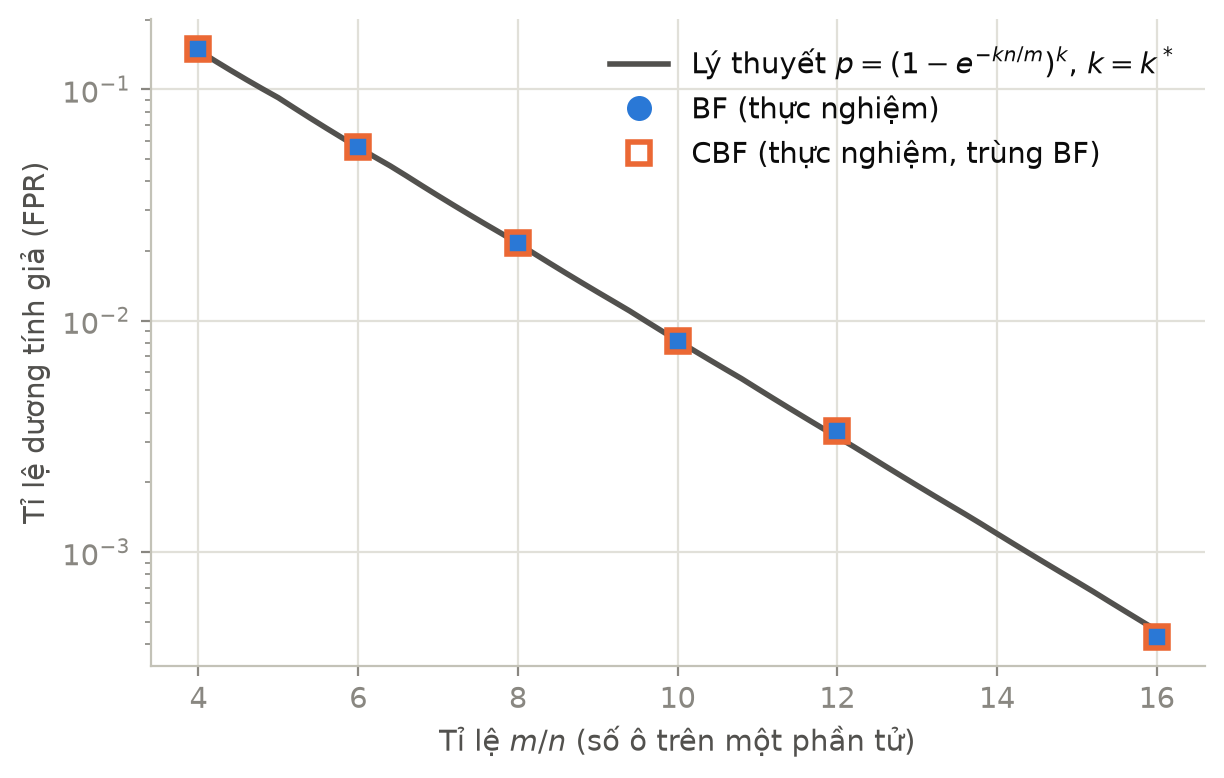
\includegraphics[width=0.72\textwidth]{fig/fpr_vs_mn.png}
\caption{FPR theo $m/n$ (trục tung log). BF và CBF trùng nhau; thanh sai số
là KTC Wilson 95\%, đường liền là $p=(1-e^{-kn/m})^k$ tại $k=k^*$.}
\label{fig:fpr_mn}
\end{figure}

\subsection{Số hàm băm tối ưu (H4)}
Hình~\ref{fig:fpr_k} quét $k$ từ 1 đến 12 tại $m/n=10$: FPR đạt cực tiểu
quanh $k^*=\KOptTen{}$ đúng như công thức~(\ref{eq:kopt}). Cơ chế: $k$ quá
nhỏ cho một khóa lạ quá ít phép thử độc lập nên hiếm cơ hội bắt gặp được
một bit 0; $k$ quá lớn làm đầy mảng bit khiến từng phép thử dễ trúng bit 1
hơn.

\begin{figure}[H]\centering
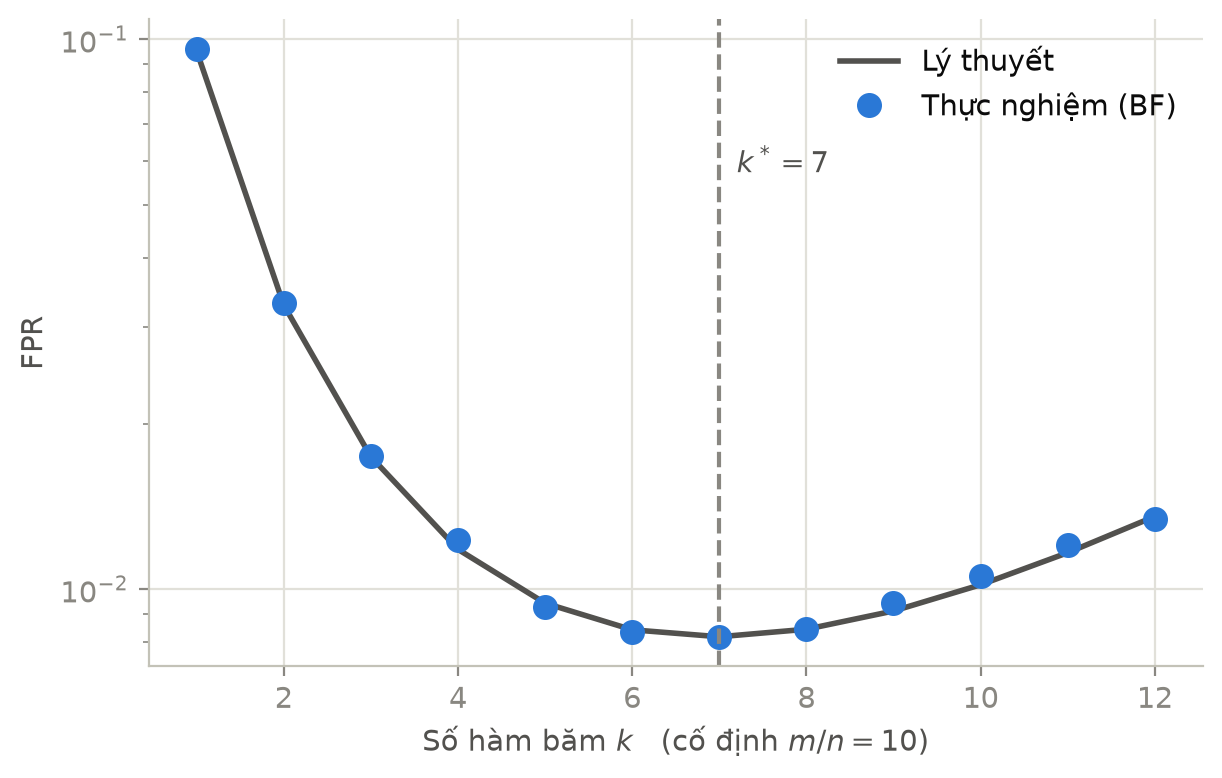
\includegraphics[width=0.72\textwidth]{fig/fpr_vs_k.png}
\caption{FPR theo số hàm băm $k$ tại $m/n=10$: cực tiểu tại
$k^*=(m/n)\ln 2\approx 7$.}
\label{fig:fpr_k}
\end{figure}

\subsection{Bộ nhớ: CBF trả giá \texorpdfstring{$4\times$}{4×} (H2)}
Bảng~\ref{tab:memory} xác nhận dung lượng payload của mảng backing: CBF 4-bit
(nibble packing) tốn đúng $4.0\times$ BF ở mọi cấu hình; CBF 8-bit tốn
$8\times$. Tại $m/n=10$: BF dùng \MemBFTen{} byte, CBF 4-bit
\MemCBFFourTen{} byte, CBF 8-bit \MemCBFEightTen{} byte. Các số này không bao
gồm object header, allocator hay RSS của tiến trình; hệ số $4\times/8\times$
được suy ra trực tiếp từ cách biểu diễn, không phải một phát hiện về runtime.

\begin{table}[H]\centering
\caption{E1: Dung lượng payload của mảng backing theo $m/n$ ($n=\NKeys{}$)}
\label{tab:memory}
\begin{tabular}{@{}rrrrrr@{}}
\toprule
$m/n$ & $m$ (ô) & BF (byte) & CBF 4-bit (byte) & CBF 8-bit (byte) & CBF4/BF\\
\midrule
4 & 400\,000 & 50\,000 & 200\,000 & 400\,000 & 4.0$\times$\\
6 & 600\,000 & 75\,000 & 300\,000 & 600\,000 & 4.0$\times$\\
8 & 800\,000 & 100\,000 & 400\,000 & 800\,000 & 4.0$\times$\\
10 & 1\,000\,000 & 125\,000 & 500\,000 & 1\,000\,000 & 4.0$\times$\\
12 & 1\,200\,000 & 150\,000 & 600\,000 & 1\,200\,000 & 4.0$\times$\\
16 & 1\,600\,000 & 200\,000 & 800\,000 & 1\,600\,000 & 4.0$\times$\\
\bottomrule
\end{tabular}

\end{table}

\subsection{Thông lượng (H3)}
\begin{table}[H]\centering
\caption{E1: Median throughput qua \BenchRepeats{} lượt
(nghìn thao tác/giây; CBF4 = CBF 4-bit)}
\label{tab:throughput}
\begin{tabular}{@{}rrrrrrrr@{}}
\toprule
$m/n$ & $k$ & \multicolumn{2}{c}{Insert} & \multicolumn{2}{c}{Query (miss)} & \multicolumn{2}{c}{Query (hit) / Delete}\\
\cmidrule(lr){3-4}\cmidrule(lr){5-6}\cmidrule(l){7-8}
 & & BF & CBF4 & BF & CBF4 & BF hit & CBF4 del\\
\midrule
4 & 3 & 1\,523 & 871 & 1\,449 & 1\,228 & 1\,211 & 863\\
6 & 4 & 1\,307 & 692 & 1\,360 & 1\,200 & 1\,054 & 678\\
8 & 6 & 1\,021 & 500 & 1\,309 & 1\,154 & 815 & 499\\
10 & 7 & 900 & 409 & 1\,364 & 1\,168 & 723 & 401\\
12 & 8 & 770 & 385 & 1\,408 & 1\,111 & 654 & 371\\
16 & 11 & 625 & 293 & 1\,411 & 1\,104 & 543 & 288\\
\bottomrule
\end{tabular}

\end{table}

Tại $m/n=10$ (Bảng~\ref{tab:throughput}, Hình~\ref{fig:throughput}): BF đạt
\InsBFTen{} nghìn insert/s so với \InsCBFTen{} của CBF 4-bit (nhanh gấp
\InsRatioTen{} lần) vì CBF phải đọc--sửa--ghi nibble thay vì chỉ bật bit.
Với query trên khóa vắng mặt, BF đạt \QmissBFTen{} nghìn thao tác/s so với
\QmissCBFTen{} của CBF (gấp \QmissRatioTen{} lần). Query trên khóa vắng mặt
(miss) nhanh hơn trên khóa có mặt (hit): với BF là \QmissBFTen{} so với
\QhitBFTen{} nghìn thao tác/s, vì truy vấn miss thoát sớm ngay khi gặp bit 0
đầu tiên, còn truy vấn hit luôn phải thăm đủ $k$ vị trí.
Delete chuẩn của CBF 4-bit đạt \DelCBFTen{} nghìn thao tác/s; phép đo giả định
caller biết khóa đã chèn và không cộng thêm một lượt Query. Mỗi điểm là median
của \BenchRepeats{} lượt, dải tô trên Hình~\ref{fig:throughput} là IQR. Các số
và tỉ số phản ánh bản cài đặt cụ thể dùng \texttt{bitarray}/\texttt{bytearray},
thao tác nibble và vòng lặp Python; chúng không chứng minh mọi cài đặt BF luôn
nhanh hơn mọi cài đặt CBF.

Hai xu hướng trong Bảng~\ref{tab:throughput} đáng bình luận thêm. Thứ nhất,
throughput của \emph{mọi} thao tác giảm dần theo $m/n$: nguyên nhân không
phải kích thước mảng mà là $k=\mathrm{round}((m/n)\ln 2)$ tăng theo, khiến
mỗi thao tác phải băm và thăm nhiều vị trí hơn; đây là chi phí ít được
đề cập của việc hạ FPR bằng cách tăng $m/n$. Thứ hai, trong nội bộ CBF, bản
8-bit nhanh hơn bản 4-bit ở mọi thao tác vì không phải tách/ghép nibble,
nhưng tốn gấp đôi bộ nhớ: ngay trong một họ cấu trúc cũng tồn tại đánh đổi
tốc độ--dung lượng, và lựa chọn 4-bit của Fan \emph{et al.} là điểm cân
bằng nghiêng về bộ nhớ.

\begin{figure}[H]\centering
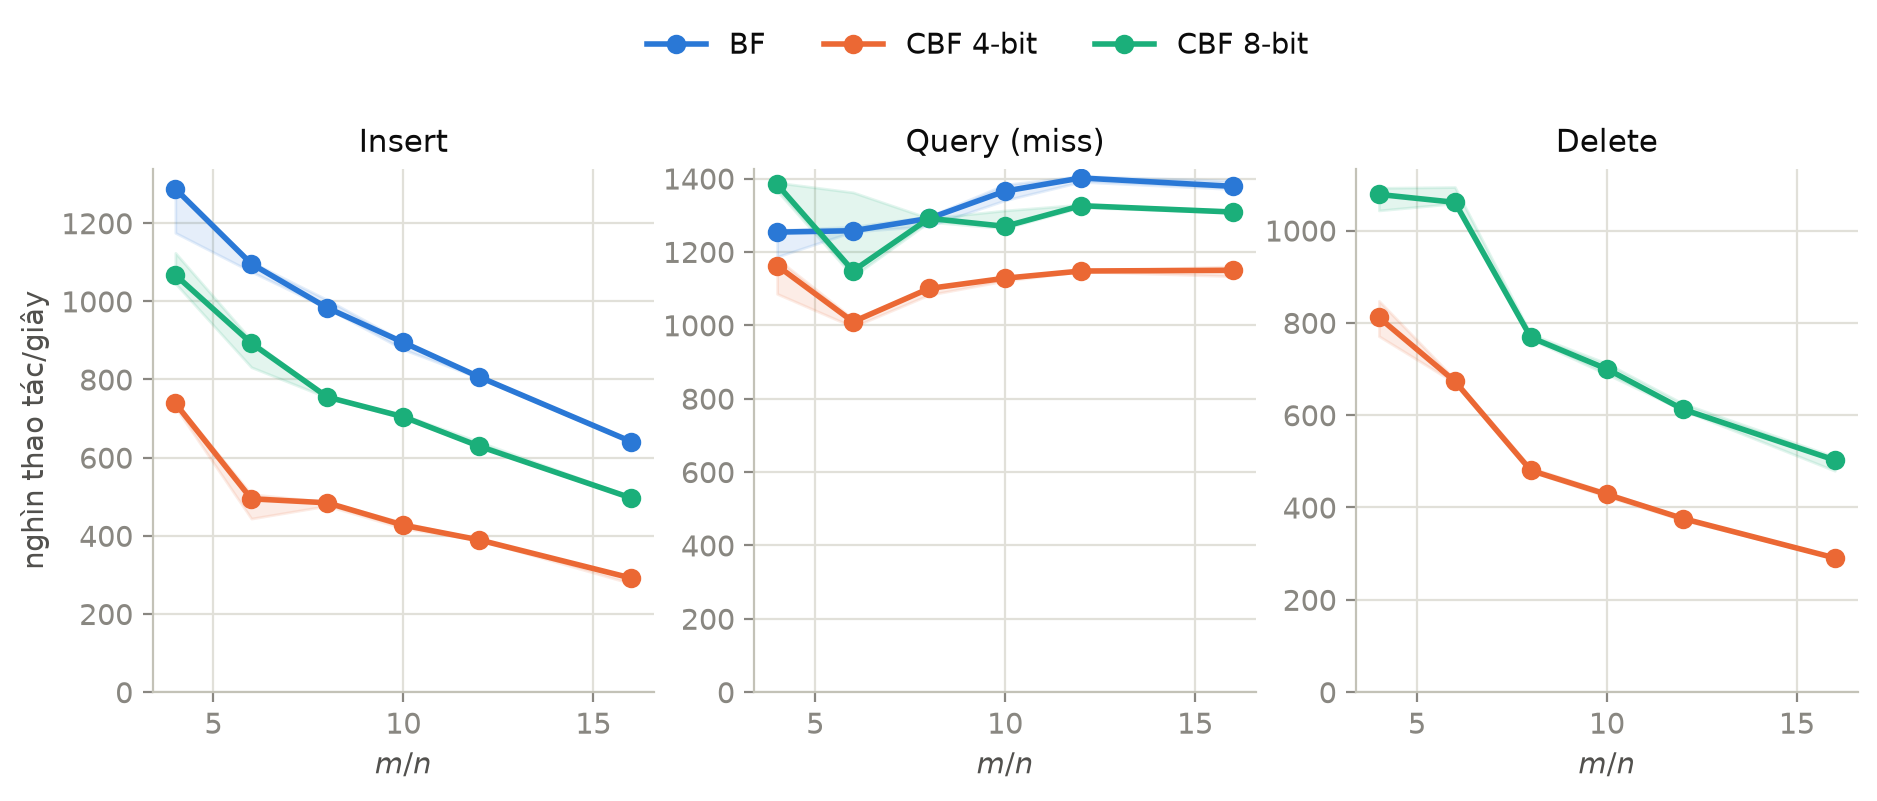
\includegraphics[width=\textwidth]{fig/throughput.png}
\caption{Median throughput insert, query (miss) và delete theo $m/n$; dải tô
là IQR của \BenchRepeats{} lượt đo.}
\label{fig:throughput}
\end{figure}

\subsection{Đánh đổi FPR khi cố định payload bộ nhớ}
\label{sec:equalbudget}
Khi dung lượng payload là ràng buộc cứng (ví dụ SRAM on-chip), phép so này
cho thấy chi phí FPR của counter; nó không làm hai cấu trúc tương đương chức
năng vì BF không hỗ trợ delete. Với cùng \BudgetBytes{} byte
(Bảng~\ref{tab:equalbudget},
Hình~\ref{fig:equalbudget}): BF có \EqCellsBF{} ô nên FPR chỉ \EqFprBF{};
CBF 4-bit còn \EqCellsCBFFour{} ô, FPR vọt lên \EqFprCBFFour{}; CBF 8-bit
còn \EqCellsCBFEight{} ô, FPR \EqFprCBFEight{}. Khoảng cách
\EqRatioFour{}--\EqRatioEight{} lần (từ hơn một tới gần hai bậc độ lớn) là
đánh đổi dung lượng--FPR để có counter và khả năng xóa.

Kết quả đo cũng được lý thuyết tiên đoán trọn vẹn: với $250\,000$ ô và
$k=2$, công thức~(\ref{eq:fpr}) cho $30.3\%$ trong khi giá trị đo là $30.1\%$; với
$125\,000$ ô và $k=1$: lý thuyết $55.1\%$, đo $54.9\%$
(Bảng~\ref{tab:equalbudget}). Nói cách khác, chi phí FPR của counter có thể
được tiên lượng đầy đủ ngay từ khâu thiết kế mà không cần đo đạc.

\begin{table}[H]\centering
\caption{E3: Cùng payload \BudgetBytes{} byte, $n=\NKeys{}$,
$k$ tối ưu cho từng cấu trúc}
\label{tab:equalbudget}
\begin{tabular}{@{}lrrrrr@{}}
\toprule
Cấu trúc & Số ô & bit/ô & $k$ & FPR lý thuyết & FPR thực nghiệm\\
\midrule
BF & 1\,000\,000 & 1 & 7 & 0.819\% & 0.819\%\\
CBF 4-bit & 250\,000 & 4 & 2 & 30.3\% & 30.1\%\\
CBF 8-bit & 125\,000 & 8 & 1 & 55.1\% & 54.9\%\\
\bottomrule
\end{tabular}

\end{table}

\begin{figure}[H]\centering
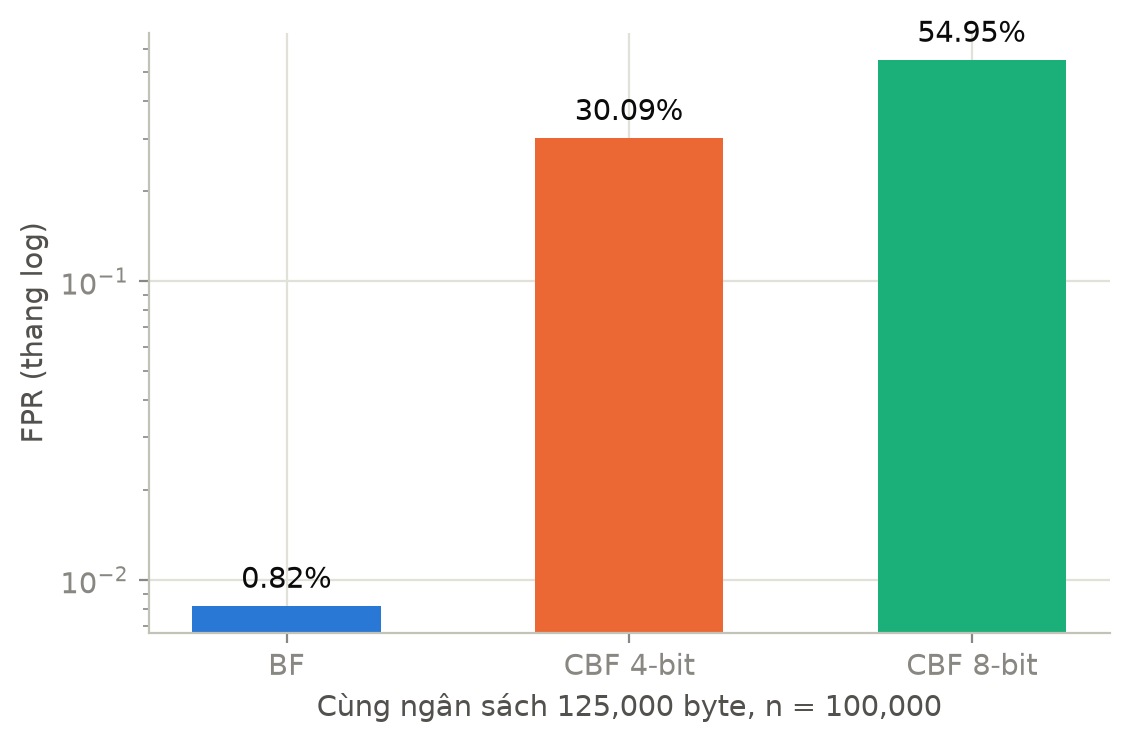
\includegraphics[width=0.62\textwidth]{fig/equal_budget.png}
\caption{FPR (thang log) khi cả ba mảng backing dùng cùng payload byte.}
\label{fig:equalbudget}
\end{figure}

\subsection{Contract của delete và stress test xóa sai}
E4 (Bảng~\ref{tab:falseneg}) trước hết kiểm tra trường hợp dùng đúng: tại
$m/n=\FnRatio{}$, counter lớn nhất sau insert chỉ là \FnMaxCounter{} nên không
có overflow; sau khi xóa đúng \FnValidDeleted{} khóa, cả
\FnValidRemaining{} khóa thật còn lại vẫn được Query nhận ra
(\FnValidFalseNeg{} false negative).

Phần hai dùng một bộ lọc riêng đã chèn đủ $n=\NKeys{}$ khóa (chưa xóa khóa
nào) và cố ý vi phạm contract của delete: hệ thống nhầm câu trả lời ``có thể
có'' là bằng chứng membership và thử xóa \FnFpDeleted{} khóa chưa từng được
chèn. Dù dùng Query guard, \FnPerformed{} yêu cầu vẫn lọt qua vì chính các khóa
này là false positive. Các lần giảm nhầm counter làm \FnCount{} phần tử thật
(\FnRate{} của $n$) biến mất khỏi bộ lọc. Đây là kết quả có điều kiện của
stress test với hàng nghìn yêu cầu xóa sai, \emph{không phải} tỉ lệ false
negative mặc định của CBF và không được tổng quát hóa sang workload dùng đúng. Biện pháp chính là chỉ xóa khóa
được xác nhận từ nguồn dữ liệu chuẩn; rebuild giúp khôi phục nếu contract hoặc
thông tin counter đã bị phá vỡ.

Về cơ chế, quy mô thiệt hại là ước lượng được: \FnPerformed{} lần xóa lọt
qua guard, mỗi lần giảm $k=6$ counter, tổng cộng $12\,246$ lần giảm sai.
Ở cấu hình $m/n=8$, trung bình mỗi ô gánh $\lambda=kn/m=0.75$ lượt băm của
khóa thật, nên mỗi lần giảm sai có xác suất đáng kể đưa một counter đang
phục vụ khóa thật về 0; số lần giảm ở quy mô này vì vậy ảnh hưởng tới nhiều
nghìn khóa, và con số \FnCount{} (\FnRate{}) phù hợp với bậc độ lớn kỳ
vọng. Rủi ro vận hành không nằm ở thiệt hại tức thời mà ở tính
\emph{tích lũy}: mỗi chu kỳ xóa sai tiếp tục làm suy giảm bộ lọc, và không
có cơ chế tự phục hồi nào ngoài việc rebuild.

\begin{table}[H]\centering
\caption{E4: Xóa đúng và stress test xóa sai trong CBF}
\label{tab:falseneg}
\small
\begin{tabular}{@{}lr@{}}
\toprule
Đại lượng & Giá trị\\
\midrule
Cấu hình & $m/n=8$, $k=6$, $n=100\,000$\\
Counter lớn nhất sau insert & 8\\
Xóa đúng / FN trong khóa thật còn lại & 20\,000 / 0\\
Khóa vắng mặt bị báo nhầm ``có'' (false positive) & 2\,164\\
Lần xóa sai lọt qua query guard & 2\,041\\
Phần tử thật bị mất trong stress test & 8\,063\\
Tỉ lệ false negative trong stress test & 8.063\%\\
\bottomrule
\end{tabular}

\end{table}

\subsection{Đối chiếu với các biến thể (E5)}
\label{sec:e5result}
Để đặt BF/CBF cạnh các thiết kế hiện đại hơn, E5 cài đặt thêm Blocked Bloom
Filter và Cuckoo Filter rồi so sánh ở cùng mức ${\approx}10$ bit/khóa
(Bảng~\ref{tab:variants}, Hình~\ref{fig:variants}); cơ chế của từng biến
thể được trình bày ở Mục~\ref{sec:variants}.

Blocked BF với block 512~bit đạt FPR \BlkFprTen{} so với \FprEmpTen{} của
BF chuẩn cùng $m,k$: phần thuế FPR trả cho tính cục bộ cache là có thật
nhưng nhỏ. Trong cài đặt phần cứng hoặc C/C++, một cache miss mỗi truy vấn
thay vì tối đa $k$ thường bù lại xứng đáng; lợi ích này nằm ngoài phạm vi
đo của Python.

Cuckoo Filter (fingerprint $f=8$~bit, bucket 4 chỗ, $2^{15}$ bucket) chèn
đủ \NKeys{} khóa không thất bại lần nào (hệ số tải \CkLoad{}), đạt FPR
\CkFpr{} với payload \CkMem{}~byte (\CkBitsPerKey{} bit/khóa), và xóa toàn
bộ khóa thành công (\CkLeftover{} khóa sót lại). Điểm đáng chú ý nhất khi
đặt cạnh nhau: trong các cấu trúc \emph{hỗ trợ xóa}, Cuckoo Filter cho FPR
thấp hơn CBF 4-bit hơn một bậc độ lớn (\CkFpr{} so với \EqFprCBFFour{});
điều này củng cố bằng số đo cho khuyến nghị ưu tiên Cuckoo Filter khi cần
xóa với yêu cầu FPR chặt. Ba lưu ý về phạm vi: payload của Cuckoo là danh nghĩa
($f$ bit mỗi chỗ); hệ số tải mới đạt \CkLoad{}, chưa ép tới ngưỡng
${\sim}95\%$; và bản cài đặt chưa dùng semi-sorting nên chưa phản ánh cấu
hình tối ưu không gian của công trình gốc~\cite{cuckoo2014}.

\begin{table}[H]\centering
\caption{E5: Năm cấu trúc ở cùng mức ${\approx}10$ bit/khóa ($n=\NKeys{}$)}
\label{tab:variants}
\begin{tabular}{@{}lrrlr@{}}
\toprule
Cấu trúc & Payload (byte) & bit/khóa & Hỗ trợ xóa & FPR đo\\
\midrule
BF & 125\,000 & 10.00 & Không & 0.819\%\\
Blocked BF & 125\,056 & 10.00 & Không & 1.163\%\\
CBF 4-bit & 125\,000 & 10.00 & Có & 30.1\%\\
CBF 8-bit & 125\,000 & 10.00 & Có & 54.9\%\\
Cuckoo Filter ($f=8$) & 131\,072 & 10.49 & Có & 2.320\%\\
\bottomrule
\end{tabular}

\end{table}

\begin{figure}[H]\centering
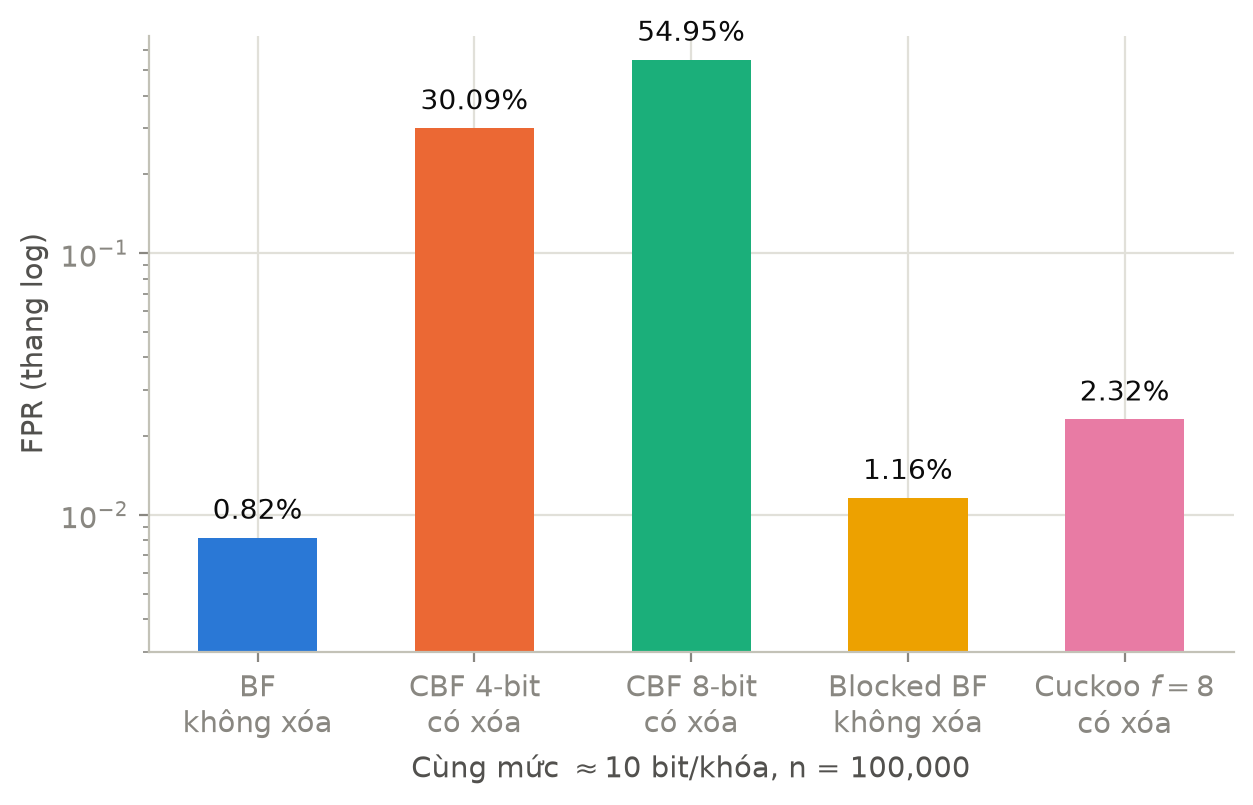
\includegraphics[width=0.8\textwidth]{fig/variants.png}
\caption{FPR (thang log) của năm cấu trúc ở cùng mức ${\approx}10$
bit/khóa; nhãn dưới mỗi cột cho biết cấu trúc có hỗ trợ xóa hay không.}
\label{fig:variants}
\end{figure}

\section{Các biến thể liên quan}
\label{sec:variants}
Ba biến thể dưới đây lần lượt khắc phục các hạn chế khác nhau của cặp
BF/CBF: chi phí cache miss, chi phí bộ nhớ của khả năng xóa, và cả hai yếu
tố cùng lúc. Cơ chế của từng biến thể được minh họa trong các
Hình~\ref{fig:blocked-diagram}--\ref{fig:dlcbf-diagram}; hai biến thể đầu
đã được đối chiếu bằng số đo trong Mục~\ref{sec:e5result}.

\subsection{Blocked Bloom Filter}
Putze \emph{et al.}~\cite{putze2010} nhận xét rằng với bộ lọc lớn hơn
cache, $k$ lần thăm bit là $k$ lần truy cập bộ nhớ ngẫu nhiên, nghĩa là tối đa
$k$ cache miss mỗi truy vấn. Blocked Bloom Filter chia mảng thành các block
bằng đúng một cache line (thường $B=512$~bit): một hàm băm phụ $h_0$ chọn
block, rồi toàn bộ $k$ bit của khóa được đặt \emph{bên trong} block đó
(Hình~\ref{fig:blocked-diagram}). Mỗi truy vấn vì vậy chỉ chạm đúng một
cache line: số cache miss giảm từ tối đa $k$ xuống ${\sim}1$, và mọi
phép thử sau lần nạp đầu tiên đều diễn ra trên thanh ghi/cache L1.

\begin{figure}[H]\centering
\begin{tikzpicture}[font=\small, >=Stealth,
    cell/.style={draw=black!55, minimum width=0.40cm, minimum height=0.40cm,
                 inner sep=0pt, fill=white},
    on/.style={cell, fill=vizblue}]
  \node[anchor=west, font=\small\bfseries] at (-1.6, 1.45) {BF chuẩn};
  \foreach \i in {0,...,15} \node[cell] (a\i) at (0.44*\i, 0) {};
  \foreach \i in {2,8,13} \node[on] at (a\i) {};
  \node[font=\small] (ka) at (-1.0, 0.75) {$x$};
  \draw[->, vizorange] (ka) to[bend left=12] (a2.north);
  \draw[->, vizorange] (ka) to[bend left=14] (a8.north);
  \draw[->, vizorange] (ka) to[bend left=16] (a13.north);
  \node[anchor=west, font=\footnotesize, text=black!60] at (7.35, 0.02)
        {$k$ vị trí rải khắp mảng};

  \begin{scope}[yshift=-2.6cm]
  \node[anchor=west, font=\small\bfseries] at (-1.6, 1.45) {Blocked BF};
  \foreach \i in {0,...,15} \node[cell] (b\i) at (0.44*\i, 0) {};
  \foreach \i in {4,8,12} \draw[black, line width=1.1pt]
        (0.44*\i - 0.22, -0.22) -- (0.44*\i - 0.22, 0.22);
  \foreach \i in {4,5,7} \node[on] at (b\i) {};
  \draw[vizblue, very thick]
        (0.44*4 - 0.21, -0.245) rectangle (0.44*8 - 0.235, 0.245);
  \node[font=\small] (kb) at (-1.0, 0.75) {$x$};
  \draw[->, vizorange] (kb) to[bend left=10] (b5.north);
  \node[font=\scriptsize, text=vizorange] at (1.0, 1.0) {$h_0$ chọn block};
  \node[anchor=west, font=\footnotesize, text=black!60] at (7.35, 0.02)
        {$k$ vị trí trong một cache line};
  \end{scope}
\end{tikzpicture}
\caption{Blocked Bloom Filter: thay vì rải $k$ bit khắp mảng (trên), toàn
bộ $k$ bit của một khóa nằm gọn trong block 512~bit do $h_0$ chọn (dưới), nên mỗi truy vấn tốn tối đa một cache miss.}
\label{fig:blocked-diagram}
\end{figure}

Chi phí đánh đổi nằm ở sự mất cân bằng tải: số khóa rơi vào một block xấp
xỉ Poisson với kỳ vọng $nB/m$, nên luôn có block nhận nhiều khóa hơn mức
trung bình và trở nên dày đặc hơn. Vì FPR là hàm lồi của tải, trung bình
FPR trên các block cao hơn FPR của bộ lọc cân bằng hoàn hảo (bất đẳng thức
Jensen); đây chính là phần chênh 1.16\% so với 0.82\% mà E5 đo được
(Mục~\ref{sec:e5result}); trong thực tế người ta bù bằng cách cấp thêm một
lượng nhỏ bit cho mỗi khóa. RocksDB dùng đúng chiến lược cache-line-local
này trong full filter~\cite{rocksdbBloom}. Như BF gốc, cấu trúc này không
hỗ trợ xóa.

\subsection{Cuckoo Filter}
Cuckoo Filter~\cite{cuckoo2014} khác biệt căn bản với mô hình mảng bit: mỗi
khóa được đại diện bằng một \emph{fingerprint} $f$~bit lưu tường minh trong
bảng băm cuckoo gồm các bucket $b$ chỗ (thường $b=4$). Mỗi khóa có đúng hai
bucket ứng viên, xác định bằng sơ đồ \emph{partial-key cuckoo hashing}
(Hình~\ref{fig:cuckoo-diagram}):
\begin{equation*}
i_1 = h(x), \qquad i_2 = i_1 \oplus h(\mathrm{fp}(x)),
\end{equation*}
trong đó phép XOR có tính đối hợp: từ bucket đang chứa fingerprint bất kỳ
luôn tính được bucket thay thế \emph{mà không cần khóa gốc}; đây là điều kiện
thiết yếu để dời chỗ (eviction) hoạt động khi bảng chỉ lưu fingerprint.

\begin{figure}[H]\centering
\begin{tikzpicture}[font=\small, >=Stealth,
    slot/.style={draw=black!55, minimum width=0.64cm, minimum height=0.40cm,
                 inner sep=0pt, font=\scriptsize, fill=white}]
  \foreach \b in {0,...,7} {
    \foreach \s in {0,...,3}
      \node[slot] (s\b-\s) at (0.68*\b, -0.44*\s) {};
    \node[font=\scriptsize, text=black!60] at (0.68*\b, 0.40) {\b};
  }
  \node[slot, fill=black!8] at (s0-0) {6E};
  \node[slot, fill=black!8] at (s1-2) {B2};
  \node[slot, fill=black!8] at (s3-1) {17};
  \node[slot, fill=black!8] at (s5-0) {D4};
  \node[slot, fill=black!8] at (s2-0) {5F};
  \node[slot, fill=vizorange!35] at (s2-1) {A7};
  \foreach \s/\v in {0/3C, 1/91, 2/C4, 3/0B}
      \node[slot, fill=black!8] at (s6-\s) {\v};
  \draw[vizblue, very thick]
        (0.68*2-0.33, -0.44*3-0.21) rectangle (0.68*2+0.33, 0.21);
  \draw[vizblue, very thick]
        (0.68*6-0.33, -0.44*3-0.21) rectangle (0.68*6+0.33, 0.21);
  \node[draw=black!55, align=left, font=\scriptsize, anchor=north]
        (keyinfo) at (1.4, -2.35)
        {khóa $x$:\quad $\mathrm{fp}=\mathrm{A7}$\\
         $i_1=h(x)=2$\\ $i_2=2\oplus h(\mathrm{A7})=6$};
  \draw[->, vizorange] (keyinfo.north) to[bend left=8] (s2-3.south);
  \draw[->, vizorange] (keyinfo.east) to[bend right=25] (s6-3.south);
  \draw[->, dashed, black!60] (s6-0.east) to[bend left=30] ++(1.35, 0.85);
  \node[font=\scriptsize, text=black!60, align=left, anchor=west]
        at (5.35, 1.35)
        {nếu cả hai bucket đầy: đuổi 3C\\ sang bucket thay thế của nó};
\end{tikzpicture}
\caption{Cuckoo Filter: fingerprint A7 của khóa $x$ có hai bucket ứng viên
$i_1=2$ và $i_2=6$; nó được đặt vào chỗ trống của bucket~2. Khi cả hai
bucket đầy, một fingerprint bị đuổi sang bucket thay thế của chính nó
(tính bằng XOR), lặp tối đa \texttt{MAX\_KICKS} lần.}
\label{fig:cuckoo-diagram}
\end{figure}

Truy vấn chỉ đọc hai bucket và so tối đa $2b$ fingerprint; mỗi phép so
trùng ngẫu nhiên với xác suất ${\sim}2^{-f}$, nên
$\varepsilon \approx 2b\alpha/2^{f}$ với $\alpha$ là hệ số tải. Ở cấu hình
E5 ($f=8$, $b=4$, $\alpha=76.3\%$) công thức cho ${\approx}2.4\%$, khớp số
đo \CkFpr{} (Mục~\ref{sec:e5result}). Nhờ lưu tường minh từng phần tử,
\emph{xóa được} bằng cách gỡ một bản sao fingerprint khỏi một trong hai
bucket; đáng chú ý, delete ở đây mang \emph{cùng contract} với CBF: chỉ
được xóa khóa chắc chắn đã chèn, vì gỡ fingerprint của khóa chưa chèn có
thể gỡ nhầm fingerprint trùng của khóa khác và gây false
negative~\cite{cuckoo2014}. Về không gian, chi phí là $f/\alpha$
bit/khóa; với kỹ thuật semi-sorting (tiết kiệm 1~bit mỗi fingerprint), khi
FPR mục tiêu $\varepsilon<3\%$ Cuckoo Filter cần ít bit hơn cả BF tối ưu
không gian, nghĩa là vừa hỗ trợ xóa vừa tiết kiệm không gian hơn. Nhược điểm:
bucket $b=4$ cho phép đẩy hệ số tải tới ${\sim}95\%$, nhưng vượt ngưỡng đó
thao tác chèn có thể thất bại (chuỗi dời chỗ quá dài), nên hệ thống phải
theo dõi tải và mở rộng bảng kịp thời.

\subsection{d-left Counting Bloom Filter}
dlCBF~\cite{bonomi2006} thay mảng counter thưa của CBF bằng bảng băm
d-left: bảng chia thành $d$ bảng con, mỗi phần tử băm ra một bucket ứng
viên trong \emph{mỗi} bảng con và được đặt vào bucket ít tải nhất, ưu tiên
bảng bên trái khi hòa (Hình~\ref{fig:dlcbf-diagram}). Quy tắc ``chọn nơi
ít tải trong $d$ lựa chọn'' làm tải cực đại tập trung mạnh quanh trung
bình, nên các bucket có thể định cỡ cố định mà gần như không lãng phí chỗ;
đây là một tính chất quý cho phần cứng vì $d$ bảng con truy cập được song
song với độ trễ cố định.

\begin{figure}[H]\centering
\begin{tikzpicture}[font=\small, >=Stealth,
    bucket/.style={draw=black!60, minimum width=1.78cm, minimum height=0.52cm,
                   inner sep=0pt, fill=white},
    entry/.style={draw=vizblue!50!black, minimum width=0.34cm,
                  minimum height=0.34cm, inner sep=0pt, fill=vizblue!65}]
  \foreach \t/\lbl in {0/1, 1/2, 2/3} {
    \node[font=\small\bfseries] at (2.75*\t, 0.62) {Bảng con \lbl};
    \foreach \r in {0,...,3} \node[bucket] (t\t-\r) at (2.75*\t, -0.72*\r) {};
  }
  % cac muc da luu trong bang (o vuong nho = mot muc)
  \foreach \t/\r/\p in {0/0/0, 0/1/0, 0/1/1, 0/3/0, 1/0/0, 1/2/0,
                        2/0/0, 2/1/0, 2/1/1, 2/3/0}
    \node[entry] at ($(t\t-\r.west)+(0.28+0.40*\p, 0)$) {};
  % ba bucket ung vien cua x: vien cam + nhan h_i(x)
  \foreach \t/\r/\i in {0/1/1, 1/2/2, 2/0/3} {
    \draw[vizorange, line width=1.2pt]
        ($(t\t-\r.south west)+(-0.035,-0.035)$) rectangle
        ($(t\t-\r.north east)+(0.035,0.035)$);
    \node[font=\scriptsize, text=vizorange, anchor=east, fill=white,
          inner sep=1.5pt] at ($(t\t-\r.west)+(-0.10, 0)$) {$h_{\i}(x)$};
  }
  % bucket duoc chon: vien xanh day
  \draw[vizaqua, line width=1.8pt]
      ($(t1-2.south west)+(-0.10,-0.10)$) rectangle
      ($(t1-2.north east)+(0.10,0.10)$);
  % phong to cau tao mot muc (zoom tu muc cua bucket t0-3)
  \node[draw=black!60, minimum width=1.7cm, minimum height=0.46cm,
        font=\scriptsize, fill=vizblue!10] (zfp) at (0.55, -3.55) {fingerprint};
  \node[draw=black!60, minimum width=1.0cm, minimum height=0.46cm,
        font=\scriptsize, fill=vizblue!10, anchor=west] (zct) at (zfp.east) {counter};
  \node[font=\scriptsize, text=black!60, anchor=east]
        at ($(zfp.west)+(-0.15, 0)$) {một mục gồm:};
  \draw[dashed, black!45] ($(t0-3.west)+(0.11, -0.17)$) -- (zfp.north west);
  \draw[dashed, black!45] ($(t0-3.west)+(0.45, -0.17)$) -- (zct.north east);
  % ghi chu lua chon
  \node[font=\footnotesize, align=left, anchor=west] at (3.35, -3.55)
      {tải ba bucket ứng viên: $2/1/1$\\
       $\Rightarrow$ chọn bảng con 2 (ít tải nhất,\\
       \phantom{$\Rightarrow$ }ưu tiên bảng bên trái khi hòa)};
\end{tikzpicture}
\caption{d-left CBF với $d=3$: khóa $x$ băm ra một bucket ứng viên trong
mỗi bảng con (viền cam, nhãn $h_i(x)$); mỗi ô vuông nhỏ là một mục đã lưu,
nên tải ba ứng viên là $2/1/1$ và bucket của bảng con~2 được chọn (viền
xanh). Phần phóng to cho thấy mỗi mục gồm một fingerprint kèm counter nhỏ
để hỗ trợ đếm bội và xóa.}
\label{fig:dlcbf-diagram}
\end{figure}

Mỗi ô của bucket lưu một fingerprint kèm counter nhỏ: \emph{insert} tìm
fingerprint trong các bucket ứng viên để tăng counter (phần tử trùng) hoặc
chiếm một ô trống; \emph{query} so fingerprint trên $d$ bucket ứng viên;
\emph{delete} giảm counter tương ứng. False positive chỉ phát sinh khi một
khóa lạ trùng cả bucket ứng viên lẫn fingerprint với một phần tử đã lưu.
Vì chỉ những phần tử thực sự có mặt mới chiếm chỗ (thay vì cấp counter
cho mọi ô kể cả ô trống như CBF), dlCBF đạt cùng chức năng đếm/xóa với
khoảng \emph{một nửa} không gian của CBF 4-bit~\cite{bonomi2006}. Cái giá
là logic phức tạp hơn đáng kể: bài gốc phải dùng thêm các phép hoán vị để
giữ insert/delete nhất quán khi cùng một phần tử có thể được nhìn thấy ở
các bảng con khác nhau. Đây là lý do báo cáo giữ dlCBF ở mức phân tích lý
thuyết thay vì cài đặt trong E5.

\section{Khuyến nghị lựa chọn}
\label{sec:recommend}
\begin{enumerate}
  \item \textbf{Tập tĩnh hoặc rebuild được}:\\
        (SSTable bất biến, Cache Digest, chữ ký DPI ít đổi) dùng \textbf{BF}.\\
        Chọn $m=-n\ln p/(\ln 2)^2$ và
        $k=\mathrm{round}((m/n)\ln 2)$ theo FPR mục
        tiêu $p$ (ví dụ $p=1\%\Rightarrow m/n\approx 9.6$, $k=7$).
  \item \textbf{Cần xóa động hoặc đếm bội}:\\ dùng \textbf{CBF 4-bit} khi hệ
        thống có nguồn dữ liệu chuẩn để bảo đảm chỉ xóa khóa đã chèn. Theo dõi
        overflow; rebuild từ nguồn dữ liệu chuẩn khi counter mất thông tin hoặc
        contract delete có thể đã bị vi phạm.
  \item \textbf{Cần xóa và bộ nhớ/FPR là ràng buộc chặt}: cân nhắc
        \textbf{Cuckoo Filter}, đặc biệt khi FPR mục tiêu $<3\%$, hoặc
        \textbf{dlCBF} trên phần cứng; theo dõi hệ số tải và thất bại insert.
  \item \textbf{Nghẽn vì cache miss}: chuyển sang \textbf{Blocked Bloom
        Filter}, chấp nhận FPR tăng nhẹ.
\end{enumerate}

\paragraph{Ví dụ thiết kế tham số.}
Yêu cầu: lọc $n=10^{7}$ khóa với FPR mục tiêu $p=1\%$, tập gần như tĩnh.
Áp dụng~(\ref{eq:kopt}):
\begin{equation*}
m=-\frac{n\ln(0.01)}{(\ln 2)^{2}}\approx 9.59\times10^{7}\ \text{bit}
\approx 11.4\ \text{MiB},\qquad
\frac{m}{n}\approx 9.59,\qquad
k=\mathrm{round}(9.59\ln 2)=7.
\end{equation*}
Thay lại~(\ref{eq:fpr}) để kiểm tra: FPR $=1.00\%$, đạt mục tiêu. Nếu cùng
số ô phải chuyển sang counter để xóa được: CBF 4-bit tốn $45.7$~MiB, CBF
8-bit tốn $91.4$~MiB, tức chênh lệch hơn 34~MiB so với BF chỉ để đổi lấy
thao tác delete. Do tập gần như tĩnh, lựa chọn phù hợp là BF kèm lịch rebuild;
chỉ khi xuất hiện yêu cầu xóa tức thời mới cân nhắc chi phí của CBF, hoặc
chuyển sang Cuckoo Filter nếu FPR mục tiêu vẫn ở mức chặt
(Mục~\ref{sec:variants}).

\section{Kết luận}
Thực nghiệm xác nhận bốn giả thuyết: FPR của BF/CBF trùng nhau và
bám công thức lý thuyết trong sai số lấy mẫu (H1), payload CBF 4-bit bằng
$4\times$ BF (H2), và trong cài đặt Python đang xét BF có median throughput
cao hơn CBF 4-bit ở các thao tác chung (H3); FPR giảm mũ theo $m/n$ với cực
tiểu theo $k$ tại $k^*$ (H4). Bức tranh tổng thể: \emph{CBF đạt được khả
năng xóa bằng cách đánh đổi payload counter lớn hơn và một contract delete
chặt chẽ hơn}. Khi chỉ xóa
khóa chắc chắn đã chèn và không overflow, thí nghiệm không quan sát false
negative; false negative xuất hiện trong stress test khi cố ý xóa các khóa
vắng mặt. Do đó BF phù hợp với tập tĩnh/rebuild được; CBF phù hợp với tập động
khi có nguồn dữ liệu chuẩn cho delete; và Cuckoo Filter, với FPR thấp hơn
CBF 4-bit hơn một bậc độ lớn ở cùng ngân sách trong E5, đáng được ưu tiên
khảo sát khi cần xóa
với yêu cầu FPR/bộ nhớ chặt.

\paragraph{Hạn chế.} Benchmark dùng một bản cài đặt Python cụ thể; dù đã báo
median/IQR qua \BenchRepeats{} lượt, cả số tuyệt đối lẫn tỉ số không đại diện
cho mọi bản cài đặt C/C++/phần cứng. FPR dùng một tập khóa tất định và một cặp
seed; KTC Wilson chỉ phản ánh sai số trên các truy vấn vắng mặt, chưa bao phủ
biến thiên qua nhiều họ hash/seed. Công thức~(\ref{eq:fpr}) là xấp xỉ (và là
cận dưới); với $m$ nhỏ nên đo thực nghiệm. Phân tích giả định hàm băm lý
tưởng; double hashing chỉ hợp lệ tiệm cận và môi trường đối kháng cần hàm băm
có khóa. Các số bộ nhớ chỉ là payload của mảng backing, không phải RSS. Bản
cài đặt Blocked BF và Cuckoo Filter trong E5 chỉ nhằm đối chiếu FPR và chức
năng xóa; chúng chưa tối ưu không gian (semi-sorting) lẫn tốc độ, nên không
dùng để so sánh throughput.

\begin{thebibliography}{9}
\bibitem{bloom1970} B.~H. Bloom, ``Space/time trade-offs in hash coding with
allowable errors,'' \emph{Communications of the ACM}, vol.~13, no.~7,
pp.~422--426, 1970.
\bibitem{fan2000} L.~Fan, P.~Cao, J.~Almeida, and A.~Z. Broder, ``Summary
Cache: A Scalable Wide-Area Web Cache Sharing Protocol,'' \emph{IEEE/ACM
Transactions on Networking}, vol.~8, no.~3, pp.~281--293, 2000.
\bibitem{broder2004} A.~Broder and M.~Mitzenmacher, ``Network Applications of
Bloom Filters: A Survey,'' \emph{Internet Mathematics}, vol.~1, no.~4,
pp.~485--509, 2004.
\bibitem{putze2010} F.~Putze, P.~Sanders, and J.~Singler, ``Cache-, hash-, and
space-efficient Bloom filters,'' \emph{ACM Journal of Experimental
Algorithmics}, vol.~14, 2009.
\bibitem{kirsch2008} A.~Kirsch and M.~Mitzenmacher, ``Less hashing, same
performance: Building a better Bloom filter,'' \emph{Random Structures \&
Algorithms}, vol.~33, no.~2, pp.~187--218, 2008.
\bibitem{bonomi2006} F.~Bonomi, M.~Mitzenmacher, R.~Panigrahy, S.~Singh, and
G.~Varghese, ``An Improved Construction for Counting Bloom Filters,'' in
\emph{Algorithms: ESA 2006}, LNCS 4168, pp.~684--695.
\bibitem{cuckoo2014} B.~Fan, D.~G. Andersen, M.~Kaminsky, and M.~D.
Mitzenmacher, ``Cuckoo Filter: Practically Better Than Bloom,'' in
\emph{Proc.\ 10th ACM CoNEXT}, pp.~75--88, 2014.
\bibitem{dpi2003} S.~Dharmapurikar, P.~Krishnamurthy, T.~Sproull, and
J.~Lockwood, ``Deep Packet Inspection using Parallel Bloom Filters,'' in
\emph{IEEE Hot Interconnects 11}, 2003.
\bibitem{rocksdbBloom} RocksDB,
\href{https://github.com/facebook/rocksdb/wiki/RocksDB-Bloom-Filter}
{``RocksDB Bloom Filter,''} project documentation, accessed Aug.~10, 2026.
\end{thebibliography}

\end{document}
